% Options for packages loaded elsewhere
\PassOptionsToPackage{unicode}{hyperref}
\PassOptionsToPackage{hyphens}{url}
%
\documentclass[
]{article}
\usepackage{amsmath,amssymb}
\usepackage{lmodern}
\usepackage{iftex}
\ifPDFTeX
  \usepackage[T1]{fontenc}
  \usepackage[utf8]{inputenc}
  \usepackage{textcomp} % provide euro and other symbols
\else % if luatex or xetex
  \usepackage{unicode-math}
  \defaultfontfeatures{Scale=MatchLowercase}
  \defaultfontfeatures[\rmfamily]{Ligatures=TeX,Scale=1}
\fi
% Use upquote if available, for straight quotes in verbatim environments
\IfFileExists{upquote.sty}{\usepackage{upquote}}{}
\IfFileExists{microtype.sty}{% use microtype if available
  \usepackage[]{microtype}
  \UseMicrotypeSet[protrusion]{basicmath} % disable protrusion for tt fonts
}{}
\makeatletter
\@ifundefined{KOMAClassName}{% if non-KOMA class
  \IfFileExists{parskip.sty}{%
    \usepackage{parskip}
  }{% else
    \setlength{\parindent}{0pt}
    \setlength{\parskip}{6pt plus 2pt minus 1pt}}
}{% if KOMA class
  \KOMAoptions{parskip=half}}
\makeatother
\usepackage{xcolor}
\usepackage[margin=1in]{geometry}
\usepackage{color}
\usepackage{fancyvrb}
\newcommand{\VerbBar}{|}
\newcommand{\VERB}{\Verb[commandchars=\\\{\}]}
\DefineVerbatimEnvironment{Highlighting}{Verbatim}{commandchars=\\\{\}}
% Add ',fontsize=\small' for more characters per line
\usepackage{framed}
\definecolor{shadecolor}{RGB}{248,248,248}
\newenvironment{Shaded}{\begin{snugshade}}{\end{snugshade}}
\newcommand{\AlertTok}[1]{\textcolor[rgb]{0.94,0.16,0.16}{#1}}
\newcommand{\AnnotationTok}[1]{\textcolor[rgb]{0.56,0.35,0.01}{\textbf{\textit{#1}}}}
\newcommand{\AttributeTok}[1]{\textcolor[rgb]{0.77,0.63,0.00}{#1}}
\newcommand{\BaseNTok}[1]{\textcolor[rgb]{0.00,0.00,0.81}{#1}}
\newcommand{\BuiltInTok}[1]{#1}
\newcommand{\CharTok}[1]{\textcolor[rgb]{0.31,0.60,0.02}{#1}}
\newcommand{\CommentTok}[1]{\textcolor[rgb]{0.56,0.35,0.01}{\textit{#1}}}
\newcommand{\CommentVarTok}[1]{\textcolor[rgb]{0.56,0.35,0.01}{\textbf{\textit{#1}}}}
\newcommand{\ConstantTok}[1]{\textcolor[rgb]{0.00,0.00,0.00}{#1}}
\newcommand{\ControlFlowTok}[1]{\textcolor[rgb]{0.13,0.29,0.53}{\textbf{#1}}}
\newcommand{\DataTypeTok}[1]{\textcolor[rgb]{0.13,0.29,0.53}{#1}}
\newcommand{\DecValTok}[1]{\textcolor[rgb]{0.00,0.00,0.81}{#1}}
\newcommand{\DocumentationTok}[1]{\textcolor[rgb]{0.56,0.35,0.01}{\textbf{\textit{#1}}}}
\newcommand{\ErrorTok}[1]{\textcolor[rgb]{0.64,0.00,0.00}{\textbf{#1}}}
\newcommand{\ExtensionTok}[1]{#1}
\newcommand{\FloatTok}[1]{\textcolor[rgb]{0.00,0.00,0.81}{#1}}
\newcommand{\FunctionTok}[1]{\textcolor[rgb]{0.00,0.00,0.00}{#1}}
\newcommand{\ImportTok}[1]{#1}
\newcommand{\InformationTok}[1]{\textcolor[rgb]{0.56,0.35,0.01}{\textbf{\textit{#1}}}}
\newcommand{\KeywordTok}[1]{\textcolor[rgb]{0.13,0.29,0.53}{\textbf{#1}}}
\newcommand{\NormalTok}[1]{#1}
\newcommand{\OperatorTok}[1]{\textcolor[rgb]{0.81,0.36,0.00}{\textbf{#1}}}
\newcommand{\OtherTok}[1]{\textcolor[rgb]{0.56,0.35,0.01}{#1}}
\newcommand{\PreprocessorTok}[1]{\textcolor[rgb]{0.56,0.35,0.01}{\textit{#1}}}
\newcommand{\RegionMarkerTok}[1]{#1}
\newcommand{\SpecialCharTok}[1]{\textcolor[rgb]{0.00,0.00,0.00}{#1}}
\newcommand{\SpecialStringTok}[1]{\textcolor[rgb]{0.31,0.60,0.02}{#1}}
\newcommand{\StringTok}[1]{\textcolor[rgb]{0.31,0.60,0.02}{#1}}
\newcommand{\VariableTok}[1]{\textcolor[rgb]{0.00,0.00,0.00}{#1}}
\newcommand{\VerbatimStringTok}[1]{\textcolor[rgb]{0.31,0.60,0.02}{#1}}
\newcommand{\WarningTok}[1]{\textcolor[rgb]{0.56,0.35,0.01}{\textbf{\textit{#1}}}}
\usepackage{longtable,booktabs,array}
\usepackage{calc} % for calculating minipage widths
% Correct order of tables after \paragraph or \subparagraph
\usepackage{etoolbox}
\makeatletter
\patchcmd\longtable{\par}{\if@noskipsec\mbox{}\fi\par}{}{}
\makeatother
% Allow footnotes in longtable head/foot
\IfFileExists{footnotehyper.sty}{\usepackage{footnotehyper}}{\usepackage{footnote}}
\makesavenoteenv{longtable}
\usepackage{graphicx}
\makeatletter
\def\maxwidth{\ifdim\Gin@nat@width>\linewidth\linewidth\else\Gin@nat@width\fi}
\def\maxheight{\ifdim\Gin@nat@height>\textheight\textheight\else\Gin@nat@height\fi}
\makeatother
% Scale images if necessary, so that they will not overflow the page
% margins by default, and it is still possible to overwrite the defaults
% using explicit options in \includegraphics[width, height, ...]{}
\setkeys{Gin}{width=\maxwidth,height=\maxheight,keepaspectratio}
% Set default figure placement to htbp
\makeatletter
\def\fps@figure{htbp}
\makeatother
\setlength{\emergencystretch}{3em} % prevent overfull lines
\providecommand{\tightlist}{%
  \setlength{\itemsep}{0pt}\setlength{\parskip}{0pt}}
\setcounter{secnumdepth}{-\maxdimen} % remove section numbering
\ifLuaTeX
  \usepackage{selnolig}  % disable illegal ligatures
\fi
\IfFileExists{bookmark.sty}{\usepackage{bookmark}}{\usepackage{hyperref}}
\IfFileExists{xurl.sty}{\usepackage{xurl}}{} % add URL line breaks if available
\urlstyle{same} % disable monospaced font for URLs
\hypersetup{
  pdftitle={The N400 effect when singular gendered antecedents are co-indexed with (a) himself or herself (b) themselves},
  pdfauthor={Joanna Morris},
  hidelinks,
  pdfcreator={LaTeX via pandoc}}

\title{The N400 effect when singular gendered antecedents are co-indexed
with (a) \emph{himself} or \emph{herself} (b) \emph{themselves}}
\author{Joanna Morris}
\date{2023-02-13}

\begin{document}
\maketitle

\hypertarget{overview}{%
\subsection{Overview}\label{overview}}

This document contains the code to reproduce the statistical analyses
described in \href{https://psyarxiv.com/hwzke}{Prasad and Morris
(2019)}. You can download the data and the original .Rmd file
\href{https://osf.io/2vjyp/}{here}.

This document has two sections:

\begin{enumerate}
\def\labelenumi{\arabic{enumi}.}
\setcounter{enumi}{1}
\tightlist
\item
  \protect\hyperlink{gender}{Analysis 1: The N400 effect when
  antecedents are co-indexed with \emph{himself} or \emph{herself}}
\item
  \protect\hyperlink{number}{Analysis 2: The N400 effect when
  antecedents are co-indexed with \emph{themselves}}
\end{enumerate}

\hypertarget{define-functions-set-parameters-and-load}{%
\subsection{Define functions, set parameters and
load}\label{define-functions-set-parameters-and-load}}

Define standard error of mean function

\begin{Shaded}
\begin{Highlighting}[]
\NormalTok{sem }\OtherTok{\textless{}{-}} \ControlFlowTok{function}\NormalTok{(x) }\FunctionTok{sd}\NormalTok{(x)}\SpecialCharTok{/}\FunctionTok{sqrt}\NormalTok{(}\FunctionTok{length}\NormalTok{(x))}
\end{Highlighting}
\end{Shaded}

Before we begin, let's set some general parameters for \texttt{ggplot2}.
We will set a general theme using the \texttt{theme\_set()} function. We
will use the `classic' theme which gives us clean white background
rather than the default grey with white grid lines. And we will position
the legend at the top of the graph rather than at the right side which
is the default.

Then we re-order factor levels for \emph{Anteriority} \&
\emph{Referentiality}

\begin{verbatim}
## [1] "Frontal"        "FrontoCentral"  "Central"        "CentroParietal"
## [5] "Parietal"
\end{verbatim}

\begin{verbatim}
## [1] "Referential"    "NonReferential"
\end{verbatim}

\begin{verbatim}
## [1] "Frontal"        "FrontoCentral"  "Central"        "CentroParietal"
## [5] "Parietal"
\end{verbatim}

\begin{verbatim}
## [1] "Referential"    "NonReferential"
\end{verbatim}

\hypertarget{analysis-1-the-n400-effect-when-antecedents-are-co-indexed-with-himself-or-herself}{%
\subsection{\texorpdfstring{Analysis 1: The N400 effect when antecedents
are co-indexed with \emph{himself} or
\emph{herself}}{Analysis 1: The N400 effect when antecedents are co-indexed with himself or herself}}\label{analysis-1-the-n400-effect-when-antecedents-are-co-indexed-with-himself-or-herself}}

\begin{Shaded}
\begin{Highlighting}[]
\FunctionTok{ezANOVA}\NormalTok{(}\AttributeTok{data =}\NormalTok{ prost\_2022\_singular}
\NormalTok{              , }\AttributeTok{dv =}\NormalTok{ diff\_score}
\NormalTok{              , }\AttributeTok{wid =}\NormalTok{ SubjID}
\NormalTok{              , }\AttributeTok{within =}\NormalTok{ .(Referentiality, Gender\_Status, Anteriority)}
\NormalTok{              , }\AttributeTok{between =}\NormalTok{ Group}
\NormalTok{              , }\AttributeTok{type =} \DecValTok{3}
\NormalTok{              , }\AttributeTok{return\_aov =}\NormalTok{ F}
\NormalTok{              )}
\end{Highlighting}
\end{Shaded}

\begin{verbatim}
## $ANOVA
##                                            Effect DFn DFd          F
## 2                                           Group   1  36  0.9374869
## 3                                  Referentiality   1  36 12.2247770
## 5                                   Gender_Status   1  36  1.2733561
## 7                                     Anteriority   4 144  2.0606903
## 4                            Group:Referentiality   1  36  0.6762734
## 6                             Group:Gender_Status   1  36  0.4610781
## 8                               Group:Anteriority   4 144  5.1495811
## 9                    Referentiality:Gender_Status   1  36  0.2476607
## 11                     Referentiality:Anteriority   4 144  1.3854470
## 13                      Gender_Status:Anteriority   4 144  2.3525738
## 10             Group:Referentiality:Gender_Status   1  36  5.7351452
## 12               Group:Referentiality:Anteriority   4 144  0.7584705
## 14                Group:Gender_Status:Anteriority   4 144  0.9712661
## 15       Referentiality:Gender_Status:Anteriority   4 144  0.2095779
## 16 Group:Referentiality:Gender_Status:Anteriority   4 144  1.4910541
##               p p<.05          ges
## 2  0.3393852751       0.0061153894
## 3  0.0012717043     * 0.0725639615
## 5  0.2666022045       0.0060391927
## 7  0.0890226513       0.0029742361
## 4  0.4162867596       0.0043096566
## 6  0.5014630657       0.0021952289
## 8  0.0006605669     * 0.0073995058
## 9  0.6217533918       0.0012878955
## 11 0.2419070474       0.0016448157
## 13 0.0567931874       0.0032557088
## 10 0.0219567998     * 0.0289966816
## 12 0.5539661827       0.0009011341
## 14 0.4252771122       0.0013467020
## 15 0.9327769406       0.0001698395
## 16 0.2079557263       0.0012070793
## 
## $`Mauchly's Test for Sphericity`
##                                            Effect           W            p
## 7                                     Anteriority 0.006548926 2.246469e-32
## 8                               Group:Anteriority 0.006548926 2.246469e-32
## 11                     Referentiality:Anteriority 0.003281484 2.660831e-37
## 12               Group:Referentiality:Anteriority 0.003281484 2.660831e-37
## 13                      Gender_Status:Anteriority 0.004635292 7.771205e-35
## 14                Group:Gender_Status:Anteriority 0.004635292 7.771205e-35
## 15       Referentiality:Gender_Status:Anteriority 0.021467327 5.607135e-24
## 16 Group:Referentiality:Gender_Status:Anteriority 0.021467327 5.607135e-24
##    p<.05
## 7      *
## 8      *
## 11     *
## 12     *
## 13     *
## 14     *
## 15     *
## 16     *
## 
## $`Sphericity Corrections`
##                                            Effect       GGe      p[GG]
## 7                                     Anteriority 0.3117498 0.15462251
## 8                               Group:Anteriority 0.3117498 0.02136772
## 11                     Referentiality:Anteriority 0.3014694 0.25188259
## 12               Group:Referentiality:Anteriority 0.3014694 0.41205819
## 13                      Gender_Status:Anteriority 0.3071411 0.12683261
## 14                Group:Gender_Status:Anteriority 0.3071411 0.34769438
## 15       Referentiality:Gender_Status:Anteriority 0.3635434 0.73986510
## 16 Group:Referentiality:Gender_Status:Anteriority 0.3635434 0.23423883
##    p[GG]<.05       HFe      p[HF] p[HF]<.05
## 7            0.3175191 0.15407353          
## 8          * 0.3175191 0.02074207         *
## 11           0.3062118 0.25222426          
## 12           0.3062118 0.41392595          
## 13           0.3124468 0.12615449          
## 14           0.3124468 0.34904640          
## 15           0.3748964 0.74703892          
## 16           0.3748964 0.23426338
\end{verbatim}

\hypertarget{condition-means-for-analysis-1}{%
\subsubsection{Condition Means for Analysis
1}\label{condition-means-for-analysis-1}}

The N400 effect when antecedents are co-indexed with \emph{himself} or
\emph{herself}.

Significant Effects: \textbf{Referentiality; Group X Anteriority; Group
x Referentiality x Gender Status}

\begin{longtable}[]{@{}lrrrrr@{}}
\toprule()
Referentiality & Mean & SE & SD & Max & Min \\
\midrule()
\endhead
Referential & -0.66 & 0.10 & 1.99 & 6.30 & -5.21 \\
NonReferential & 0.36 & 0.09 & 1.74 & 4.79 & -5.06 \\
\bottomrule()
\end{longtable}

\begin{longtable}[]{@{}llrrrrr@{}}
\toprule()
Anteriority & Group & Mean & SE & SD & Max & Min \\
\midrule()
\endhead
Frontal & Binary & -0.12 & 0.27 & 2.43 & 6.30 & -5.05 \\
Frontal & NonBinary & -0.31 & 0.25 & 2.15 & 3.88 & -5.21 \\
FrontoCentral & Binary & -0.25 & 0.23 & 2.04 & 4.41 & -4.97 \\
FrontoCentral & NonBinary & -0.21 & 0.22 & 1.87 & 3.47 & -5.13 \\
Central & Binary & -0.39 & 0.21 & 1.87 & 4.39 & -5.12 \\
Central & NonBinary & 0.01 & 0.21 & 1.77 & 4.27 & -4.49 \\
CentroParietal & Binary & -0.38 & 0.21 & 1.84 & 3.93 & -4.73 \\
CentroParietal & NonBinary & 0.15 & 0.21 & 1.74 & 4.44 & -4.67 \\
Parietal & Binary & -0.28 & 0.20 & 1.79 & 4.11 & -5.06 \\
Parietal & NonBinary & 0.36 & 0.20 & 1.72 & 3.76 & -4.75 \\
\bottomrule()
\end{longtable}

\begin{longtable}[]{@{}
  >{\raggedright\arraybackslash}p{(\columnwidth - 14\tabcolsep) * \real{0.2273}}
  >{\raggedright\arraybackslash}p{(\columnwidth - 14\tabcolsep) * \real{0.2121}}
  >{\raggedright\arraybackslash}p{(\columnwidth - 14\tabcolsep) * \real{0.1515}}
  >{\raggedleft\arraybackslash}p{(\columnwidth - 14\tabcolsep) * \real{0.0909}}
  >{\raggedleft\arraybackslash}p{(\columnwidth - 14\tabcolsep) * \real{0.0758}}
  >{\raggedleft\arraybackslash}p{(\columnwidth - 14\tabcolsep) * \real{0.0758}}
  >{\raggedleft\arraybackslash}p{(\columnwidth - 14\tabcolsep) * \real{0.0758}}
  >{\raggedleft\arraybackslash}p{(\columnwidth - 14\tabcolsep) * \real{0.0909}}@{}}
\toprule()
\begin{minipage}[b]{\linewidth}\raggedright
Referentiality
\end{minipage} & \begin{minipage}[b]{\linewidth}\raggedright
Gender\_Status
\end{minipage} & \begin{minipage}[b]{\linewidth}\raggedright
Group
\end{minipage} & \begin{minipage}[b]{\linewidth}\raggedleft
Mean
\end{minipage} & \begin{minipage}[b]{\linewidth}\raggedleft
SE
\end{minipage} & \begin{minipage}[b]{\linewidth}\raggedleft
SD
\end{minipage} & \begin{minipage}[b]{\linewidth}\raggedleft
Max
\end{minipage} & \begin{minipage}[b]{\linewidth}\raggedleft
Min
\end{minipage} \\
\midrule()
\endhead
Referential & Gendered & Binary & -1.51 & 0.19 & 1.90 & 4.41 & -5.12 \\
Referential & Gendered & NonBinary & -0.20 & 0.21 & 2.03 & 4.44 &
-5.21 \\
Referential & NonGendered & Binary & -0.31 & 0.21 & 2.11 & 6.30 &
-5.05 \\
Referential & NonGendered & NonBinary & -0.58 & 0.17 & 1.63 & 3.22 &
-4.75 \\
NonReferential & Gendered & Binary & 0.49 & 0.16 & 1.64 & 3.90 &
-4.58 \\
NonReferential & Gendered & NonBinary & 0.08 & 0.18 & 1.71 & 3.76 &
-3.19 \\
NonReferential & NonGendered & Binary & 0.19 & 0.17 & 1.73 & 4.79 &
-5.06 \\
NonReferential & NonGendered & NonBinary & 0.69 & 0.20 & 1.85 & 3.88 &
-4.12 \\
\bottomrule()
\end{longtable}

\hypertarget{post-hoc-tests-for-analysis-1-group-x-gender-status-x-referentiality}{%
\subsubsection{Post-hoc tests for Analysis 1: Group x Gender Status x
Referentiality}\label{post-hoc-tests-for-analysis-1-group-x-gender-status-x-referentiality}}

The following chunk runs post-hoc tests for the 3-way
\textbf{\emph{``Group x Gender Status x Referentiality''}} Interaction

\hypertarget{binary-group.}{%
\paragraph{Binary Group.}\label{binary-group.}}

These are the post-hoc tests for the \emph{binary} group.

``\emph{Some woman\ldots himself}'' vs.~``\emph{Mary\ldots himself}''
Binary

\begin{Shaded}
\begin{Highlighting}[]
\FunctionTok{pander}\NormalTok{(}\FunctionTok{t.test}\NormalTok{(diff\_score }\SpecialCharTok{\textasciitilde{}}\NormalTok{ Referentiality}
\NormalTok{       , }\FunctionTok{filter}\NormalTok{(binary, (Gender\_Status }\SpecialCharTok{==} \StringTok{"Gendered"}\NormalTok{))}
\NormalTok{       , }\AttributeTok{paired=}\ConstantTok{TRUE}\NormalTok{))}
\end{Highlighting}
\end{Shaded}

\begin{longtable}[]{@{}
  >{\centering\arraybackslash}p{(\columnwidth - 8\tabcolsep) * \real{0.2048}}
  >{\centering\arraybackslash}p{(\columnwidth - 8\tabcolsep) * \real{0.0602}}
  >{\centering\arraybackslash}p{(\columnwidth - 8\tabcolsep) * \real{0.2169}}
  >{\centering\arraybackslash}p{(\columnwidth - 8\tabcolsep) * \real{0.3012}}
  >{\centering\arraybackslash}p{(\columnwidth - 8\tabcolsep) * \real{0.2169}}@{}}
\caption{Paired t-test: \texttt{diff\_score} by
\texttt{Referentiality}}\tabularnewline
\toprule()
\begin{minipage}[b]{\linewidth}\centering
Test statistic
\end{minipage} & \begin{minipage}[b]{\linewidth}\centering
df
\end{minipage} & \begin{minipage}[b]{\linewidth}\centering
P value
\end{minipage} & \begin{minipage}[b]{\linewidth}\centering
Alternative hypothesis
\end{minipage} & \begin{minipage}[b]{\linewidth}\centering
mean difference
\end{minipage} \\
\midrule()
\endfirsthead
\toprule()
\begin{minipage}[b]{\linewidth}\centering
Test statistic
\end{minipage} & \begin{minipage}[b]{\linewidth}\centering
df
\end{minipage} & \begin{minipage}[b]{\linewidth}\centering
P value
\end{minipage} & \begin{minipage}[b]{\linewidth}\centering
Alternative hypothesis
\end{minipage} & \begin{minipage}[b]{\linewidth}\centering
mean difference
\end{minipage} \\
\midrule()
\endhead
-7.66 & 99 & 1.275e-11 * * * & two.sided & -2.007 \\
\bottomrule()
\end{longtable}

``\emph{Someone\ldots himself}'' vs.~``\emph{The
participant\ldots himself}'' Binary

\begin{Shaded}
\begin{Highlighting}[]
\FunctionTok{pander}\NormalTok{(}\FunctionTok{t.test}\NormalTok{(diff\_score }\SpecialCharTok{\textasciitilde{}}\NormalTok{ Referentiality}
\NormalTok{       , }\FunctionTok{filter}\NormalTok{(binary, (Gender\_Status }\SpecialCharTok{==} \StringTok{"NonGendered"}\NormalTok{))}
\NormalTok{       , }\AttributeTok{paired=}\ConstantTok{TRUE}\NormalTok{))}
\end{Highlighting}
\end{Shaded}

\begin{longtable}[]{@{}
  >{\centering\arraybackslash}p{(\columnwidth - 8\tabcolsep) * \real{0.2267}}
  >{\centering\arraybackslash}p{(\columnwidth - 8\tabcolsep) * \real{0.0667}}
  >{\centering\arraybackslash}p{(\columnwidth - 8\tabcolsep) * \real{0.1333}}
  >{\centering\arraybackslash}p{(\columnwidth - 8\tabcolsep) * \real{0.3333}}
  >{\centering\arraybackslash}p{(\columnwidth - 8\tabcolsep) * \real{0.2400}}@{}}
\caption{Paired t-test: \texttt{diff\_score} by
\texttt{Referentiality}}\tabularnewline
\toprule()
\begin{minipage}[b]{\linewidth}\centering
Test statistic
\end{minipage} & \begin{minipage}[b]{\linewidth}\centering
df
\end{minipage} & \begin{minipage}[b]{\linewidth}\centering
P value
\end{minipage} & \begin{minipage}[b]{\linewidth}\centering
Alternative hypothesis
\end{minipage} & \begin{minipage}[b]{\linewidth}\centering
mean difference
\end{minipage} \\
\midrule()
\endfirsthead
\toprule()
\begin{minipage}[b]{\linewidth}\centering
Test statistic
\end{minipage} & \begin{minipage}[b]{\linewidth}\centering
df
\end{minipage} & \begin{minipage}[b]{\linewidth}\centering
P value
\end{minipage} & \begin{minipage}[b]{\linewidth}\centering
Alternative hypothesis
\end{minipage} & \begin{minipage}[b]{\linewidth}\centering
mean difference
\end{minipage} \\
\midrule()
\endhead
-1.722 & 99 & 0.08825 & two.sided & -0.4954 \\
\bottomrule()
\end{longtable}

``\emph{The participant\ldots himself}''
vs.~``\emph{Mary\ldots himself}'' Binary

\begin{Shaded}
\begin{Highlighting}[]
\FunctionTok{pander}\NormalTok{(}\FunctionTok{t.test}\NormalTok{(diff\_score }\SpecialCharTok{\textasciitilde{}}\NormalTok{ Gender\_Status}
\NormalTok{       , }\FunctionTok{filter}\NormalTok{(binary, (Referentiality }\SpecialCharTok{==} \StringTok{"Referential"}\NormalTok{))}
\NormalTok{       , }\AttributeTok{paired=}\ConstantTok{TRUE}\NormalTok{))}
\end{Highlighting}
\end{Shaded}

\begin{longtable}[]{@{}
  >{\centering\arraybackslash}p{(\columnwidth - 8\tabcolsep) * \real{0.2048}}
  >{\centering\arraybackslash}p{(\columnwidth - 8\tabcolsep) * \real{0.0602}}
  >{\centering\arraybackslash}p{(\columnwidth - 8\tabcolsep) * \real{0.2169}}
  >{\centering\arraybackslash}p{(\columnwidth - 8\tabcolsep) * \real{0.3012}}
  >{\centering\arraybackslash}p{(\columnwidth - 8\tabcolsep) * \real{0.2169}}@{}}
\caption{Paired t-test: \texttt{diff\_score} by
\texttt{Gender\_Status}}\tabularnewline
\toprule()
\begin{minipage}[b]{\linewidth}\centering
Test statistic
\end{minipage} & \begin{minipage}[b]{\linewidth}\centering
df
\end{minipage} & \begin{minipage}[b]{\linewidth}\centering
P value
\end{minipage} & \begin{minipage}[b]{\linewidth}\centering
Alternative hypothesis
\end{minipage} & \begin{minipage}[b]{\linewidth}\centering
mean difference
\end{minipage} \\
\midrule()
\endfirsthead
\toprule()
\begin{minipage}[b]{\linewidth}\centering
Test statistic
\end{minipage} & \begin{minipage}[b]{\linewidth}\centering
df
\end{minipage} & \begin{minipage}[b]{\linewidth}\centering
P value
\end{minipage} & \begin{minipage}[b]{\linewidth}\centering
Alternative hypothesis
\end{minipage} & \begin{minipage}[b]{\linewidth}\centering
mean difference
\end{minipage} \\
\midrule()
\endhead
-4.909 & 99 & 3.612e-06 * * * & two.sided & -1.208 \\
\bottomrule()
\end{longtable}

``\emph{Someone\ldots himself}'' vs.~``\emph{Some woman\ldots himself}''
Binary

\begin{Shaded}
\begin{Highlighting}[]
\FunctionTok{pander}\NormalTok{(}\FunctionTok{t.test}\NormalTok{(diff\_score }\SpecialCharTok{\textasciitilde{}}\NormalTok{ Gender\_Status}
\NormalTok{       , }\FunctionTok{filter}\NormalTok{(binary, (Referentiality }\SpecialCharTok{==} \StringTok{"NonReferential"}\NormalTok{))}
\NormalTok{       , }\AttributeTok{paired=}\ConstantTok{TRUE}\NormalTok{))}
\end{Highlighting}
\end{Shaded}

\begin{longtable}[]{@{}
  >{\centering\arraybackslash}p{(\columnwidth - 8\tabcolsep) * \real{0.2267}}
  >{\centering\arraybackslash}p{(\columnwidth - 8\tabcolsep) * \real{0.0667}}
  >{\centering\arraybackslash}p{(\columnwidth - 8\tabcolsep) * \real{0.1333}}
  >{\centering\arraybackslash}p{(\columnwidth - 8\tabcolsep) * \real{0.3333}}
  >{\centering\arraybackslash}p{(\columnwidth - 8\tabcolsep) * \real{0.2400}}@{}}
\caption{Paired t-test: \texttt{diff\_score} by
\texttt{Gender\_Status}}\tabularnewline
\toprule()
\begin{minipage}[b]{\linewidth}\centering
Test statistic
\end{minipage} & \begin{minipage}[b]{\linewidth}\centering
df
\end{minipage} & \begin{minipage}[b]{\linewidth}\centering
P value
\end{minipage} & \begin{minipage}[b]{\linewidth}\centering
Alternative hypothesis
\end{minipage} & \begin{minipage}[b]{\linewidth}\centering
mean difference
\end{minipage} \\
\midrule()
\endfirsthead
\toprule()
\begin{minipage}[b]{\linewidth}\centering
Test statistic
\end{minipage} & \begin{minipage}[b]{\linewidth}\centering
df
\end{minipage} & \begin{minipage}[b]{\linewidth}\centering
P value
\end{minipage} & \begin{minipage}[b]{\linewidth}\centering
Alternative hypothesis
\end{minipage} & \begin{minipage}[b]{\linewidth}\centering
mean difference
\end{minipage} \\
\midrule()
\endhead
1.248 & 99 & 0.2148 & two.sided & 0.3037 \\
\bottomrule()
\end{longtable}

``\emph{Someone\ldots himself}'' vs.~``\emph{Mary\ldots himself}''
Binary

\begin{Shaded}
\begin{Highlighting}[]
\NormalTok{mary\_someone }\OtherTok{\textless{}{-}} \FunctionTok{filter}\NormalTok{(binary, (Referentiality }\SpecialCharTok{==} \StringTok{"Referential"} \SpecialCharTok{\&}\NormalTok{ Gender\_Status }\SpecialCharTok{==} \StringTok{"Gendered"}\NormalTok{) }\SpecialCharTok{|}\NormalTok{ (Referentiality }\SpecialCharTok{==} \StringTok{"NonReferential"} \SpecialCharTok{\&}\NormalTok{ Gender\_Status }\SpecialCharTok{==} \StringTok{"NonGendered"}\NormalTok{))}

\FunctionTok{pander}\NormalTok{(}\FunctionTok{t.test}\NormalTok{(diff\_score }\SpecialCharTok{\textasciitilde{}}\NormalTok{ Gender\_Status, mary\_someone, }\AttributeTok{paired=}\ConstantTok{TRUE}\NormalTok{))}
\end{Highlighting}
\end{Shaded}

\begin{longtable}[]{@{}
  >{\centering\arraybackslash}p{(\columnwidth - 8\tabcolsep) * \real{0.2073}}
  >{\centering\arraybackslash}p{(\columnwidth - 8\tabcolsep) * \real{0.0610}}
  >{\centering\arraybackslash}p{(\columnwidth - 8\tabcolsep) * \real{0.2073}}
  >{\centering\arraybackslash}p{(\columnwidth - 8\tabcolsep) * \real{0.3049}}
  >{\centering\arraybackslash}p{(\columnwidth - 8\tabcolsep) * \real{0.2195}}@{}}
\caption{Paired t-test: \texttt{diff\_score} by
\texttt{Gender\_Status}}\tabularnewline
\toprule()
\begin{minipage}[b]{\linewidth}\centering
Test statistic
\end{minipage} & \begin{minipage}[b]{\linewidth}\centering
df
\end{minipage} & \begin{minipage}[b]{\linewidth}\centering
P value
\end{minipage} & \begin{minipage}[b]{\linewidth}\centering
Alternative hypothesis
\end{minipage} & \begin{minipage}[b]{\linewidth}\centering
mean difference
\end{minipage} \\
\midrule()
\endfirsthead
\toprule()
\begin{minipage}[b]{\linewidth}\centering
Test statistic
\end{minipage} & \begin{minipage}[b]{\linewidth}\centering
df
\end{minipage} & \begin{minipage}[b]{\linewidth}\centering
P value
\end{minipage} & \begin{minipage}[b]{\linewidth}\centering
Alternative hypothesis
\end{minipage} & \begin{minipage}[b]{\linewidth}\centering
mean difference
\end{minipage} \\
\midrule()
\endhead
-6.88 & 99 & 5.47e-10 * * * & two.sided & -1.704 \\
\bottomrule()
\end{longtable}

``\emph{Some woman\ldots himself}'' vs.~``\emph{the
participant\ldots himself}'' Binary

\begin{longtable}[]{@{}
  >{\centering\arraybackslash}p{(\columnwidth - 8\tabcolsep) * \real{0.2208}}
  >{\centering\arraybackslash}p{(\columnwidth - 8\tabcolsep) * \real{0.0649}}
  >{\centering\arraybackslash}p{(\columnwidth - 8\tabcolsep) * \real{0.1558}}
  >{\centering\arraybackslash}p{(\columnwidth - 8\tabcolsep) * \real{0.3247}}
  >{\centering\arraybackslash}p{(\columnwidth - 8\tabcolsep) * \real{0.2338}}@{}}
\caption{Paired t-test: \texttt{diff\_score} by
\texttt{Gender\_Status}}\tabularnewline
\toprule()
\begin{minipage}[b]{\linewidth}\centering
Test statistic
\end{minipage} & \begin{minipage}[b]{\linewidth}\centering
df
\end{minipage} & \begin{minipage}[b]{\linewidth}\centering
P value
\end{minipage} & \begin{minipage}[b]{\linewidth}\centering
Alternative hypothesis
\end{minipage} & \begin{minipage}[b]{\linewidth}\centering
mean difference
\end{minipage} \\
\midrule()
\endfirsthead
\toprule()
\begin{minipage}[b]{\linewidth}\centering
Test statistic
\end{minipage} & \begin{minipage}[b]{\linewidth}\centering
df
\end{minipage} & \begin{minipage}[b]{\linewidth}\centering
P value
\end{minipage} & \begin{minipage}[b]{\linewidth}\centering
Alternative hypothesis
\end{minipage} & \begin{minipage}[b]{\linewidth}\centering
mean difference
\end{minipage} \\
\midrule()
\endhead
2.594 & 99 & 0.01094 * & two.sided & 0.7992 \\
\bottomrule()
\end{longtable}

\hypertarget{interaction-plots-group-x-gender-status-x-referentiality-binary}{%
\subparagraph{Interaction Plots: Group x Gender Status x Referentiality
Binary}\label{interaction-plots-group-x-gender-status-x-referentiality-binary}}

~

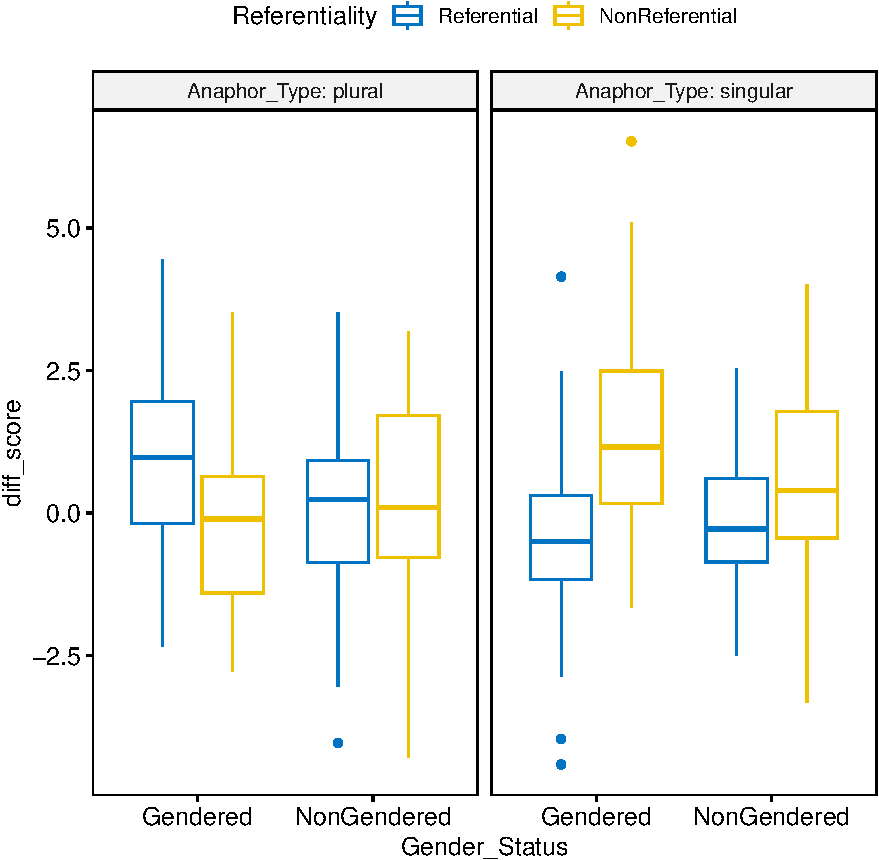
\includegraphics{prost_2022_n400_nref_b_files/figure-latex/unnamed-chunk-13-1.pdf}

~

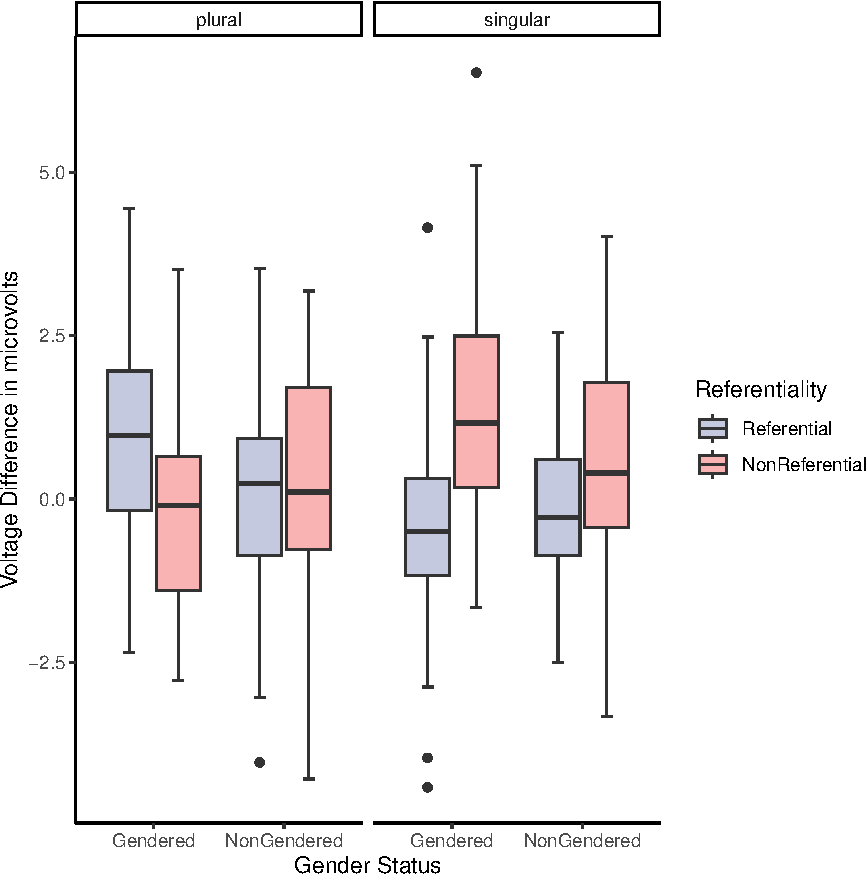
\includegraphics{prost_2022_n400_nref_b_files/figure-latex/unnamed-chunk-14-1.pdf}

\hypertarget{nonbinary-group.}{%
\paragraph{NonBinary Group.}\label{nonbinary-group.}}

These are the post-hoc tests for the \emph{NonBinary} group.

``\emph{Some woman\ldots himself}'' vs.~``\emph{Mary\ldots himself}''
NonBinary

\begin{Shaded}
\begin{Highlighting}[]
\FunctionTok{pander}\NormalTok{(}\FunctionTok{t.test}\NormalTok{(diff\_score }\SpecialCharTok{\textasciitilde{}}\NormalTok{ Referentiality}
\NormalTok{       ,}\FunctionTok{filter}\NormalTok{(prost\_2022\_singular, (Gender\_Status }\SpecialCharTok{==} \StringTok{"Gendered"} \SpecialCharTok{\&}\NormalTok{ Group }\SpecialCharTok{==} \StringTok{"NonBinary"}\NormalTok{))}
\NormalTok{       ,}\AttributeTok{paired=}\ConstantTok{TRUE}\NormalTok{))}
\end{Highlighting}
\end{Shaded}

\begin{longtable}[]{@{}
  >{\centering\arraybackslash}p{(\columnwidth - 8\tabcolsep) * \real{0.2267}}
  >{\centering\arraybackslash}p{(\columnwidth - 8\tabcolsep) * \real{0.0667}}
  >{\centering\arraybackslash}p{(\columnwidth - 8\tabcolsep) * \real{0.1333}}
  >{\centering\arraybackslash}p{(\columnwidth - 8\tabcolsep) * \real{0.3333}}
  >{\centering\arraybackslash}p{(\columnwidth - 8\tabcolsep) * \real{0.2400}}@{}}
\caption{Paired t-test: \texttt{diff\_score} by
\texttt{Referentiality}}\tabularnewline
\toprule()
\begin{minipage}[b]{\linewidth}\centering
Test statistic
\end{minipage} & \begin{minipage}[b]{\linewidth}\centering
df
\end{minipage} & \begin{minipage}[b]{\linewidth}\centering
P value
\end{minipage} & \begin{minipage}[b]{\linewidth}\centering
Alternative hypothesis
\end{minipage} & \begin{minipage}[b]{\linewidth}\centering
mean difference
\end{minipage} \\
\midrule()
\endfirsthead
\toprule()
\begin{minipage}[b]{\linewidth}\centering
Test statistic
\end{minipage} & \begin{minipage}[b]{\linewidth}\centering
df
\end{minipage} & \begin{minipage}[b]{\linewidth}\centering
P value
\end{minipage} & \begin{minipage}[b]{\linewidth}\centering
Alternative hypothesis
\end{minipage} & \begin{minipage}[b]{\linewidth}\centering
mean difference
\end{minipage} \\
\midrule()
\endhead
-1.143 & 89 & 0.2562 & two.sided & -0.279 \\
\bottomrule()
\end{longtable}

``\emph{Someone\ldots himself}'' vs.~``\emph{The
participant\ldots himself}'' NonBinary

\begin{Shaded}
\begin{Highlighting}[]
\FunctionTok{pander}\NormalTok{(}\FunctionTok{t.test}\NormalTok{(diff\_score }\SpecialCharTok{\textasciitilde{}}\NormalTok{ Referentiality}
\NormalTok{       , }\FunctionTok{filter}\NormalTok{(prost\_2022\_singular, (Gender\_Status }\SpecialCharTok{==} \StringTok{"NonGendered"} \SpecialCharTok{\&}\NormalTok{ Group }\SpecialCharTok{==} \StringTok{"NonBinary"}\NormalTok{))}
\NormalTok{       , }\AttributeTok{paired=}\ConstantTok{TRUE}\NormalTok{))}
\end{Highlighting}
\end{Shaded}

\begin{longtable}[]{@{}
  >{\centering\arraybackslash}p{(\columnwidth - 8\tabcolsep) * \real{0.2048}}
  >{\centering\arraybackslash}p{(\columnwidth - 8\tabcolsep) * \real{0.0602}}
  >{\centering\arraybackslash}p{(\columnwidth - 8\tabcolsep) * \real{0.2169}}
  >{\centering\arraybackslash}p{(\columnwidth - 8\tabcolsep) * \real{0.3012}}
  >{\centering\arraybackslash}p{(\columnwidth - 8\tabcolsep) * \real{0.2169}}@{}}
\caption{Paired t-test: \texttt{diff\_score} by
\texttt{Referentiality}}\tabularnewline
\toprule()
\begin{minipage}[b]{\linewidth}\centering
Test statistic
\end{minipage} & \begin{minipage}[b]{\linewidth}\centering
df
\end{minipage} & \begin{minipage}[b]{\linewidth}\centering
P value
\end{minipage} & \begin{minipage}[b]{\linewidth}\centering
Alternative hypothesis
\end{minipage} & \begin{minipage}[b]{\linewidth}\centering
mean difference
\end{minipage} \\
\midrule()
\endfirsthead
\toprule()
\begin{minipage}[b]{\linewidth}\centering
Test statistic
\end{minipage} & \begin{minipage}[b]{\linewidth}\centering
df
\end{minipage} & \begin{minipage}[b]{\linewidth}\centering
P value
\end{minipage} & \begin{minipage}[b]{\linewidth}\centering
Alternative hypothesis
\end{minipage} & \begin{minipage}[b]{\linewidth}\centering
mean difference
\end{minipage} \\
\midrule()
\endhead
-5.202 & 89 & 1.251e-06 * * * & two.sided & -1.271 \\
\bottomrule()
\end{longtable}

``\emph{The participant\ldots himself}''
vs.~``\emph{Mary\ldots himself}'' NonBinary

\begin{Shaded}
\begin{Highlighting}[]
\FunctionTok{pander}\NormalTok{(}\FunctionTok{t.test}\NormalTok{(diff\_score }\SpecialCharTok{\textasciitilde{}}\NormalTok{ Gender\_Status}
\NormalTok{       , }\FunctionTok{filter}\NormalTok{(prost\_2022\_singular, (Referentiality }\SpecialCharTok{==} \StringTok{"Referential"} \SpecialCharTok{\&}\NormalTok{ Group }\SpecialCharTok{==} \StringTok{"NonBinary"}\NormalTok{))}
\NormalTok{       , }\AttributeTok{paired=}\ConstantTok{TRUE}\NormalTok{))}
\end{Highlighting}
\end{Shaded}

\begin{longtable}[]{@{}
  >{\centering\arraybackslash}p{(\columnwidth - 8\tabcolsep) * \real{0.2267}}
  >{\centering\arraybackslash}p{(\columnwidth - 8\tabcolsep) * \real{0.0667}}
  >{\centering\arraybackslash}p{(\columnwidth - 8\tabcolsep) * \real{0.1333}}
  >{\centering\arraybackslash}p{(\columnwidth - 8\tabcolsep) * \real{0.3333}}
  >{\centering\arraybackslash}p{(\columnwidth - 8\tabcolsep) * \real{0.2400}}@{}}
\caption{Paired t-test: \texttt{diff\_score} by
\texttt{Gender\_Status}}\tabularnewline
\toprule()
\begin{minipage}[b]{\linewidth}\centering
Test statistic
\end{minipage} & \begin{minipage}[b]{\linewidth}\centering
df
\end{minipage} & \begin{minipage}[b]{\linewidth}\centering
P value
\end{minipage} & \begin{minipage}[b]{\linewidth}\centering
Alternative hypothesis
\end{minipage} & \begin{minipage}[b]{\linewidth}\centering
mean difference
\end{minipage} \\
\midrule()
\endfirsthead
\toprule()
\begin{minipage}[b]{\linewidth}\centering
Test statistic
\end{minipage} & \begin{minipage}[b]{\linewidth}\centering
df
\end{minipage} & \begin{minipage}[b]{\linewidth}\centering
P value
\end{minipage} & \begin{minipage}[b]{\linewidth}\centering
Alternative hypothesis
\end{minipage} & \begin{minipage}[b]{\linewidth}\centering
mean difference
\end{minipage} \\
\midrule()
\endhead
1.354 & 89 & 0.1791 & two.sided & 0.3834 \\
\bottomrule()
\end{longtable}

``\emph{Someone\ldots himself}'' vs.~``\emph{Some woman\ldots himself}''
NonBinary

\begin{Shaded}
\begin{Highlighting}[]
\FunctionTok{pander}\NormalTok{(}\FunctionTok{t.test}\NormalTok{(diff\_score }\SpecialCharTok{\textasciitilde{}}\NormalTok{ Gender\_Status}
\NormalTok{       , }\FunctionTok{filter}\NormalTok{(prost\_2022\_singular, (Referentiality }\SpecialCharTok{==} \StringTok{"NonReferential"} \SpecialCharTok{\&}\NormalTok{ Group }\SpecialCharTok{==} \StringTok{"NonBinary"}\NormalTok{))}
\NormalTok{       , }\AttributeTok{paired=}\ConstantTok{TRUE}\NormalTok{))}
\end{Highlighting}
\end{Shaded}

\begin{longtable}[]{@{}
  >{\centering\arraybackslash}p{(\columnwidth - 8\tabcolsep) * \real{0.2125}}
  >{\centering\arraybackslash}p{(\columnwidth - 8\tabcolsep) * \real{0.0625}}
  >{\centering\arraybackslash}p{(\columnwidth - 8\tabcolsep) * \real{0.1875}}
  >{\centering\arraybackslash}p{(\columnwidth - 8\tabcolsep) * \real{0.3125}}
  >{\centering\arraybackslash}p{(\columnwidth - 8\tabcolsep) * \real{0.2250}}@{}}
\caption{Paired t-test: \texttt{diff\_score} by
\texttt{Gender\_Status}}\tabularnewline
\toprule()
\begin{minipage}[b]{\linewidth}\centering
Test statistic
\end{minipage} & \begin{minipage}[b]{\linewidth}\centering
df
\end{minipage} & \begin{minipage}[b]{\linewidth}\centering
P value
\end{minipage} & \begin{minipage}[b]{\linewidth}\centering
Alternative hypothesis
\end{minipage} & \begin{minipage}[b]{\linewidth}\centering
mean difference
\end{minipage} \\
\midrule()
\endfirsthead
\toprule()
\begin{minipage}[b]{\linewidth}\centering
Test statistic
\end{minipage} & \begin{minipage}[b]{\linewidth}\centering
df
\end{minipage} & \begin{minipage}[b]{\linewidth}\centering
P value
\end{minipage} & \begin{minipage}[b]{\linewidth}\centering
Alternative hypothesis
\end{minipage} & \begin{minipage}[b]{\linewidth}\centering
mean difference
\end{minipage} \\
\midrule()
\endhead
-2.792 & 89 & 0.006407 * * & two.sided & -0.6082 \\
\bottomrule()
\end{longtable}

``\emph{Someone\ldots himself}'' vs.~``\emph{Mary\ldots himself}''
NonBinary

\begin{Shaded}
\begin{Highlighting}[]
\NormalTok{mary\_someone }\OtherTok{\textless{}{-}} \FunctionTok{filter}\NormalTok{(nonbinary, (Referentiality }\SpecialCharTok{==} \StringTok{"Referential"} \SpecialCharTok{\&}\NormalTok{ Gender\_Status }\SpecialCharTok{==} \StringTok{"Gendered"}\NormalTok{) }\SpecialCharTok{|}\NormalTok{ (Referentiality }\SpecialCharTok{==} \StringTok{"NonReferential"} \SpecialCharTok{\&}\NormalTok{ Gender\_Status }\SpecialCharTok{==} \StringTok{"NonGendered"}\NormalTok{))}

\FunctionTok{pander}\NormalTok{(}\FunctionTok{t.test}\NormalTok{(diff\_score }\SpecialCharTok{\textasciitilde{}}\NormalTok{ Gender\_Status, mary\_someone, }\AttributeTok{paired=}\ConstantTok{TRUE}\NormalTok{))}
\end{Highlighting}
\end{Shaded}

\begin{longtable}[]{@{}
  >{\centering\arraybackslash}p{(\columnwidth - 8\tabcolsep) * \real{0.2048}}
  >{\centering\arraybackslash}p{(\columnwidth - 8\tabcolsep) * \real{0.0602}}
  >{\centering\arraybackslash}p{(\columnwidth - 8\tabcolsep) * \real{0.2169}}
  >{\centering\arraybackslash}p{(\columnwidth - 8\tabcolsep) * \real{0.3012}}
  >{\centering\arraybackslash}p{(\columnwidth - 8\tabcolsep) * \real{0.2169}}@{}}
\caption{Paired t-test: \texttt{diff\_score} by
\texttt{Gender\_Status}}\tabularnewline
\toprule()
\begin{minipage}[b]{\linewidth}\centering
Test statistic
\end{minipage} & \begin{minipage}[b]{\linewidth}\centering
df
\end{minipage} & \begin{minipage}[b]{\linewidth}\centering
P value
\end{minipage} & \begin{minipage}[b]{\linewidth}\centering
Alternative hypothesis
\end{minipage} & \begin{minipage}[b]{\linewidth}\centering
mean difference
\end{minipage} \\
\midrule()
\endfirsthead
\toprule()
\begin{minipage}[b]{\linewidth}\centering
Test statistic
\end{minipage} & \begin{minipage}[b]{\linewidth}\centering
df
\end{minipage} & \begin{minipage}[b]{\linewidth}\centering
P value
\end{minipage} & \begin{minipage}[b]{\linewidth}\centering
Alternative hypothesis
\end{minipage} & \begin{minipage}[b]{\linewidth}\centering
mean difference
\end{minipage} \\
\midrule()
\endhead
-3.549 & 89 & 0.0006201 * * * & two.sided & -0.8872 \\
\bottomrule()
\end{longtable}

``\emph{Some woman\ldots himself}'' vs.~``\emph{the
participant\ldots himself}'' NonBinary

\begin{longtable}[]{@{}
  >{\centering\arraybackslash}p{(\columnwidth - 8\tabcolsep) * \real{0.2125}}
  >{\centering\arraybackslash}p{(\columnwidth - 8\tabcolsep) * \real{0.0625}}
  >{\centering\arraybackslash}p{(\columnwidth - 8\tabcolsep) * \real{0.1875}}
  >{\centering\arraybackslash}p{(\columnwidth - 8\tabcolsep) * \real{0.3125}}
  >{\centering\arraybackslash}p{(\columnwidth - 8\tabcolsep) * \real{0.2250}}@{}}
\caption{Paired t-test: \texttt{diff\_score} by \texttt{Gender\_Status}
\#\#\#\#\# Interaction Plots: Group x Gender Status x Referentiality
NonBinary}\tabularnewline
\toprule()
\begin{minipage}[b]{\linewidth}\centering
Test statistic
\end{minipage} & \begin{minipage}[b]{\linewidth}\centering
df
\end{minipage} & \begin{minipage}[b]{\linewidth}\centering
P value
\end{minipage} & \begin{minipage}[b]{\linewidth}\centering
Alternative hypothesis
\end{minipage} & \begin{minipage}[b]{\linewidth}\centering
mean difference
\end{minipage} \\
\midrule()
\endfirsthead
\toprule()
\begin{minipage}[b]{\linewidth}\centering
Test statistic
\end{minipage} & \begin{minipage}[b]{\linewidth}\centering
df
\end{minipage} & \begin{minipage}[b]{\linewidth}\centering
P value
\end{minipage} & \begin{minipage}[b]{\linewidth}\centering
Alternative hypothesis
\end{minipage} & \begin{minipage}[b]{\linewidth}\centering
mean difference
\end{minipage} \\
\midrule()
\endhead
2.8 & 89 & 0.006269 * * & two.sided & 0.6624 \\
\bottomrule()
\end{longtable}

~

\includegraphics{prost_2022_n400_nref_b_files/figure-latex/unnamed-chunk-22-1.pdf}

~

\includegraphics{prost_2022_n400_nref_b_files/figure-latex/unnamed-chunk-23-1.pdf}

\hypertarget{post-hoc-tests-for-analysis-1-group-x-anteriority}{%
\subsubsection{Post-hoc tests for Analysis 1: Group x
Anteriority}\label{post-hoc-tests-for-analysis-1-group-x-anteriority}}

The following chunk runs post-hoc tests for the 2-way
\textbf{\emph{``Group x Anteriority''}} Interaction

\begin{Shaded}
\begin{Highlighting}[]
\CommentTok{\# Binary vs Non{-}Binary Frontal}

\FunctionTok{pander}\NormalTok{(}\FunctionTok{t.test}\NormalTok{(diff\_score }\SpecialCharTok{\textasciitilde{}}\NormalTok{ Group}
\NormalTok{       ,dplyr}\SpecialCharTok{::}\FunctionTok{filter}\NormalTok{(prost\_2022\_singular, (Anteriority }\SpecialCharTok{==} \StringTok{"Frontal"}\NormalTok{))}
\NormalTok{       ,}\AttributeTok{paired=}\ConstantTok{FALSE}\NormalTok{))}
\end{Highlighting}
\end{Shaded}

\begin{longtable}[]{@{}
  >{\centering\arraybackslash}p{(\columnwidth - 8\tabcolsep) * \real{0.2048}}
  >{\centering\arraybackslash}p{(\columnwidth - 8\tabcolsep) * \real{0.0723}}
  >{\centering\arraybackslash}p{(\columnwidth - 8\tabcolsep) * \real{0.1205}}
  >{\centering\arraybackslash}p{(\columnwidth - 8\tabcolsep) * \real{0.3012}}
  >{\centering\arraybackslash}p{(\columnwidth - 8\tabcolsep) * \real{0.3012}}@{}}
\caption{Welch Two Sample t-test: \texttt{diff\_score} by \texttt{Group}
(continued below)}\tabularnewline
\toprule()
\begin{minipage}[b]{\linewidth}\centering
Test statistic
\end{minipage} & \begin{minipage}[b]{\linewidth}\centering
df
\end{minipage} & \begin{minipage}[b]{\linewidth}\centering
P value
\end{minipage} & \begin{minipage}[b]{\linewidth}\centering
Alternative hypothesis
\end{minipage} & \begin{minipage}[b]{\linewidth}\centering
mean in group Binary
\end{minipage} \\
\midrule()
\endfirsthead
\toprule()
\begin{minipage}[b]{\linewidth}\centering
Test statistic
\end{minipage} & \begin{minipage}[b]{\linewidth}\centering
df
\end{minipage} & \begin{minipage}[b]{\linewidth}\centering
P value
\end{minipage} & \begin{minipage}[b]{\linewidth}\centering
Alternative hypothesis
\end{minipage} & \begin{minipage}[b]{\linewidth}\centering
mean in group Binary
\end{minipage} \\
\midrule()
\endhead
0.5115 & 150 & 0.6097 & two.sided & -0.12 \\
\bottomrule()
\end{longtable}

\begin{longtable}[]{@{}
  >{\centering\arraybackslash}p{(\columnwidth - 0\tabcolsep) * \real{0.3611}}@{}}
\toprule()
\begin{minipage}[b]{\linewidth}\centering
mean in group NonBinary
\end{minipage} \\
\midrule()
\endhead
-0.3102 \\
\bottomrule()
\end{longtable}

\begin{Shaded}
\begin{Highlighting}[]
\CommentTok{\# Binary vs Non{-}Binary FrontoCentral}

\FunctionTok{pander}\NormalTok{(}\FunctionTok{t.test}\NormalTok{(diff\_score }\SpecialCharTok{\textasciitilde{}}\NormalTok{ Group}
\NormalTok{       ,dplyr}\SpecialCharTok{::}\FunctionTok{filter}\NormalTok{(prost\_2022\_singular, (Anteriority }\SpecialCharTok{==} \StringTok{"FrontoCentral"}\NormalTok{))}
\NormalTok{       ,}\AttributeTok{paired=}\ConstantTok{FALSE}\NormalTok{))}
\end{Highlighting}
\end{Shaded}

\begin{longtable}[]{@{}
  >{\centering\arraybackslash}p{(\columnwidth - 6\tabcolsep) * \real{0.2361}}
  >{\centering\arraybackslash}p{(\columnwidth - 6\tabcolsep) * \real{0.1111}}
  >{\centering\arraybackslash}p{(\columnwidth - 6\tabcolsep) * \real{0.1389}}
  >{\centering\arraybackslash}p{(\columnwidth - 6\tabcolsep) * \real{0.3472}}@{}}
\caption{Welch Two Sample t-test: \texttt{diff\_score} by \texttt{Group}
(continued below)}\tabularnewline
\toprule()
\begin{minipage}[b]{\linewidth}\centering
Test statistic
\end{minipage} & \begin{minipage}[b]{\linewidth}\centering
df
\end{minipage} & \begin{minipage}[b]{\linewidth}\centering
P value
\end{minipage} & \begin{minipage}[b]{\linewidth}\centering
Alternative hypothesis
\end{minipage} \\
\midrule()
\endfirsthead
\toprule()
\begin{minipage}[b]{\linewidth}\centering
Test statistic
\end{minipage} & \begin{minipage}[b]{\linewidth}\centering
df
\end{minipage} & \begin{minipage}[b]{\linewidth}\centering
P value
\end{minipage} & \begin{minipage}[b]{\linewidth}\centering
Alternative hypothesis
\end{minipage} \\
\midrule()
\endhead
-0.1109 & 149.9 & 0.9119 & two.sided \\
\bottomrule()
\end{longtable}

\begin{longtable}[]{@{}
  >{\centering\arraybackslash}p{(\columnwidth - 2\tabcolsep) * \real{0.3194}}
  >{\centering\arraybackslash}p{(\columnwidth - 2\tabcolsep) * \real{0.3611}}@{}}
\toprule()
\begin{minipage}[b]{\linewidth}\centering
mean in group Binary
\end{minipage} & \begin{minipage}[b]{\linewidth}\centering
mean in group NonBinary
\end{minipage} \\
\midrule()
\endhead
-0.2496 & -0.2145 \\
\bottomrule()
\end{longtable}

\begin{Shaded}
\begin{Highlighting}[]
\CommentTok{\# Binary vs Non{-}Binary Central}

\FunctionTok{pander}\NormalTok{(}\FunctionTok{t.test}\NormalTok{(diff\_score }\SpecialCharTok{\textasciitilde{}}\NormalTok{ Group}
\NormalTok{       ,dplyr}\SpecialCharTok{::}\FunctionTok{filter}\NormalTok{(prost\_2022\_singular, (Anteriority }\SpecialCharTok{==} \StringTok{"Central"}\NormalTok{))}
\NormalTok{       ,}\AttributeTok{paired=}\ConstantTok{FALSE}\NormalTok{))}
\end{Highlighting}
\end{Shaded}

\begin{longtable}[]{@{}
  >{\centering\arraybackslash}p{(\columnwidth - 6\tabcolsep) * \real{0.2361}}
  >{\centering\arraybackslash}p{(\columnwidth - 6\tabcolsep) * \real{0.1111}}
  >{\centering\arraybackslash}p{(\columnwidth - 6\tabcolsep) * \real{0.1389}}
  >{\centering\arraybackslash}p{(\columnwidth - 6\tabcolsep) * \real{0.3472}}@{}}
\caption{Welch Two Sample t-test: \texttt{diff\_score} by \texttt{Group}
(continued below)}\tabularnewline
\toprule()
\begin{minipage}[b]{\linewidth}\centering
Test statistic
\end{minipage} & \begin{minipage}[b]{\linewidth}\centering
df
\end{minipage} & \begin{minipage}[b]{\linewidth}\centering
P value
\end{minipage} & \begin{minipage}[b]{\linewidth}\centering
Alternative hypothesis
\end{minipage} \\
\midrule()
\endfirsthead
\toprule()
\begin{minipage}[b]{\linewidth}\centering
Test statistic
\end{minipage} & \begin{minipage}[b]{\linewidth}\centering
df
\end{minipage} & \begin{minipage}[b]{\linewidth}\centering
P value
\end{minipage} & \begin{minipage}[b]{\linewidth}\centering
Alternative hypothesis
\end{minipage} \\
\midrule()
\endhead
-1.359 & 149.7 & 0.1761 & two.sided \\
\bottomrule()
\end{longtable}

\begin{longtable}[]{@{}
  >{\centering\arraybackslash}p{(\columnwidth - 2\tabcolsep) * \real{0.3194}}
  >{\centering\arraybackslash}p{(\columnwidth - 2\tabcolsep) * \real{0.3611}}@{}}
\toprule()
\begin{minipage}[b]{\linewidth}\centering
mean in group Binary
\end{minipage} & \begin{minipage}[b]{\linewidth}\centering
mean in group NonBinary
\end{minipage} \\
\midrule()
\endhead
-0.3873 & 0.01419 \\
\bottomrule()
\end{longtable}

\begin{Shaded}
\begin{Highlighting}[]
\CommentTok{\# Binary vs Non{-}Binary CentroParietal}

\FunctionTok{pander}\NormalTok{(}\FunctionTok{t.test}\NormalTok{(diff\_score }\SpecialCharTok{\textasciitilde{}}\NormalTok{ Group}
\NormalTok{       ,dplyr}\SpecialCharTok{::}\FunctionTok{filter}\NormalTok{(prost\_2022\_singular, (Anteriority }\SpecialCharTok{==} \StringTok{"CentroParietal"}\NormalTok{))}
\NormalTok{       ,}\AttributeTok{paired=}\ConstantTok{FALSE}\NormalTok{))}
\end{Highlighting}
\end{Shaded}

\begin{longtable}[]{@{}
  >{\centering\arraybackslash}p{(\columnwidth - 6\tabcolsep) * \real{0.2361}}
  >{\centering\arraybackslash}p{(\columnwidth - 6\tabcolsep) * \real{0.1111}}
  >{\centering\arraybackslash}p{(\columnwidth - 6\tabcolsep) * \real{0.1389}}
  >{\centering\arraybackslash}p{(\columnwidth - 6\tabcolsep) * \real{0.3472}}@{}}
\caption{Welch Two Sample t-test: \texttt{diff\_score} by \texttt{Group}
(continued below)}\tabularnewline
\toprule()
\begin{minipage}[b]{\linewidth}\centering
Test statistic
\end{minipage} & \begin{minipage}[b]{\linewidth}\centering
df
\end{minipage} & \begin{minipage}[b]{\linewidth}\centering
P value
\end{minipage} & \begin{minipage}[b]{\linewidth}\centering
Alternative hypothesis
\end{minipage} \\
\midrule()
\endfirsthead
\toprule()
\begin{minipage}[b]{\linewidth}\centering
Test statistic
\end{minipage} & \begin{minipage}[b]{\linewidth}\centering
df
\end{minipage} & \begin{minipage}[b]{\linewidth}\centering
P value
\end{minipage} & \begin{minipage}[b]{\linewidth}\centering
Alternative hypothesis
\end{minipage} \\
\midrule()
\endhead
-1.853 & 149.6 & 0.06587 & two.sided \\
\bottomrule()
\end{longtable}

\begin{longtable}[]{@{}
  >{\centering\arraybackslash}p{(\columnwidth - 2\tabcolsep) * \real{0.3194}}
  >{\centering\arraybackslash}p{(\columnwidth - 2\tabcolsep) * \real{0.3611}}@{}}
\toprule()
\begin{minipage}[b]{\linewidth}\centering
mean in group Binary
\end{minipage} & \begin{minipage}[b]{\linewidth}\centering
mean in group NonBinary
\end{minipage} \\
\midrule()
\endhead
-0.3836 & 0.1546 \\
\bottomrule()
\end{longtable}

\begin{Shaded}
\begin{Highlighting}[]
\CommentTok{\# Binary vs Non{-}Binary Parietal}

\FunctionTok{pander}\NormalTok{(}\FunctionTok{t.test}\NormalTok{(diff\_score }\SpecialCharTok{\textasciitilde{}}\NormalTok{ Group}
\NormalTok{       ,dplyr}\SpecialCharTok{::}\FunctionTok{filter}\NormalTok{(prost\_2022\_singular, (Anteriority }\SpecialCharTok{==} \StringTok{"Parietal"}\NormalTok{))}
\NormalTok{       ,}\AttributeTok{paired=}\ConstantTok{FALSE}\NormalTok{))}
\end{Highlighting}
\end{Shaded}

\begin{longtable}[]{@{}
  >{\centering\arraybackslash}p{(\columnwidth - 6\tabcolsep) * \real{0.2361}}
  >{\centering\arraybackslash}p{(\columnwidth - 6\tabcolsep) * \real{0.1111}}
  >{\centering\arraybackslash}p{(\columnwidth - 6\tabcolsep) * \real{0.1667}}
  >{\centering\arraybackslash}p{(\columnwidth - 6\tabcolsep) * \real{0.3472}}@{}}
\caption{Welch Two Sample t-test: \texttt{diff\_score} by \texttt{Group}
(continued below)}\tabularnewline
\toprule()
\begin{minipage}[b]{\linewidth}\centering
Test statistic
\end{minipage} & \begin{minipage}[b]{\linewidth}\centering
df
\end{minipage} & \begin{minipage}[b]{\linewidth}\centering
P value
\end{minipage} & \begin{minipage}[b]{\linewidth}\centering
Alternative hypothesis
\end{minipage} \\
\midrule()
\endfirsthead
\toprule()
\begin{minipage}[b]{\linewidth}\centering
Test statistic
\end{minipage} & \begin{minipage}[b]{\linewidth}\centering
df
\end{minipage} & \begin{minipage}[b]{\linewidth}\centering
P value
\end{minipage} & \begin{minipage}[b]{\linewidth}\centering
Alternative hypothesis
\end{minipage} \\
\midrule()
\endhead
-2.229 & 149.3 & 0.02728 * & two.sided \\
\bottomrule()
\end{longtable}

\begin{longtable}[]{@{}
  >{\centering\arraybackslash}p{(\columnwidth - 2\tabcolsep) * \real{0.3194}}
  >{\centering\arraybackslash}p{(\columnwidth - 2\tabcolsep) * \real{0.3611}}@{}}
\toprule()
\begin{minipage}[b]{\linewidth}\centering
mean in group Binary
\end{minipage} & \begin{minipage}[b]{\linewidth}\centering
mean in group NonBinary
\end{minipage} \\
\midrule()
\endhead
-0.279 & 0.3568 \\
\bottomrule()
\end{longtable}

\hypertarget{interaction-plot-group-x-anteriority}{%
\subparagraph{Interaction Plot: Group x
Anteriority}\label{interaction-plot-group-x-anteriority}}

~

\includegraphics{prost_2022_n400_nref_b_files/figure-latex/unnamed-chunk-25-1.pdf}

~

~

~

\hypertarget{analysis-2-the-n400-effect-when-antecedents-are-co-indexed-with-themselves}{%
\subsection{\texorpdfstring{Analysis 2: The N400 effect when antecedents
are co-indexed with
\emph{themselves}}{Analysis 2: The N400 effect when antecedents are co-indexed with themselves}}\label{analysis-2-the-n400-effect-when-antecedents-are-co-indexed-with-themselves}}

\begin{Shaded}
\begin{Highlighting}[]
\FunctionTok{ezANOVA}\NormalTok{(}\AttributeTok{data =}\NormalTok{ prost\_2022\_plural}
\NormalTok{              , }\AttributeTok{dv =}\NormalTok{ diff\_score}
\NormalTok{              , }\AttributeTok{wid =}\NormalTok{ SubjID}
\NormalTok{              , }\AttributeTok{within =}\NormalTok{ .(Referentiality, Gender\_Status, Anteriority)}
\NormalTok{              , }\AttributeTok{between =}\NormalTok{ Group}
\NormalTok{              , }\AttributeTok{type =} \DecValTok{3}
\NormalTok{              , }\AttributeTok{return\_aov =}\NormalTok{ F}
\NormalTok{              )}
\end{Highlighting}
\end{Shaded}

\begin{verbatim}
## $ANOVA
##                                            Effect DFn DFd           F         p
## 2                                           Group   1  36 0.238003158 0.6286102
## 3                                  Referentiality   1  36 0.006154688 0.9379031
## 5                                   Gender_Status   1  36 0.097418428 0.7567506
## 7                                     Anteriority   4 144 1.400145919 0.2369032
## 4                            Group:Referentiality   1  36 0.007236331 0.9326798
## 6                             Group:Gender_Status   1  36 0.007002636 0.9337731
## 8                               Group:Anteriority   4 144 0.052760330 0.9947472
## 9                    Referentiality:Gender_Status   1  36 2.379600770 0.1316746
## 11                     Referentiality:Anteriority   4 144 1.192347966 0.3167516
## 13                      Gender_Status:Anteriority   4 144 0.867672469 0.4850282
## 10             Group:Referentiality:Gender_Status   1  36 0.046873525 0.8298179
## 12               Group:Referentiality:Anteriority   4 144 0.043204326 0.9964316
## 14                Group:Gender_Status:Anteriority   4 144 1.904147481 0.1128999
## 15       Referentiality:Gender_Status:Anteriority   4 144 0.632964163 0.6397719
## 16 Group:Referentiality:Gender_Status:Anteriority   4 144 0.102769696 0.9813708
##    p<.05          ges
## 2        1.997832e-03
## 3        3.485373e-05
## 5        4.305791e-04
## 7        9.550056e-04
## 4        4.097878e-05
## 6        3.096328e-05
## 8        3.601964e-05
## 9        1.303825e-02
## 11       1.299619e-03
## 13       8.881270e-04
## 10       2.601535e-04
## 12       4.715031e-05
## 14       1.946970e-03
## 15       5.894000e-04
## 16       9.574378e-05
## 
## $`Mauchly's Test for Sphericity`
##                                            Effect           W            p
## 7                                     Anteriority 0.016789812 1.045004e-25
## 8                               Group:Anteriority 0.016789812 1.045004e-25
## 11                     Referentiality:Anteriority 0.003911051 4.769720e-36
## 12               Group:Referentiality:Anteriority 0.003911051 4.769720e-36
## 13                      Gender_Status:Anteriority 0.003122257 1.173632e-37
## 14                Group:Gender_Status:Anteriority 0.003122257 1.173632e-37
## 15       Referentiality:Gender_Status:Anteriority 0.019213046 9.302422e-25
## 16 Group:Referentiality:Gender_Status:Anteriority 0.019213046 9.302422e-25
##    p<.05
## 7      *
## 8      *
## 11     *
## 12     *
## 13     *
## 14     *
## 15     *
## 16     *
## 
## $`Sphericity Corrections`
##                                            Effect       GGe     p[GG] p[GG]<.05
## 7                                     Anteriority 0.3526937 0.2517930          
## 8                               Group:Anteriority 0.3526937 0.8942407          
## 11                     Referentiality:Anteriority 0.3044471 0.2917829          
## 12               Group:Referentiality:Anteriority 0.3044471 0.8798835          
## 13                      Gender_Status:Anteriority 0.3064638 0.3780187          
## 14                Group:Gender_Status:Anteriority 0.3064638 0.1731027          
## 15       Referentiality:Gender_Status:Anteriority 0.3644889 0.4868838          
## 16 Group:Referentiality:Gender_Status:Anteriority 0.3644889 0.8404737          
##          HFe     p[HF] p[HF]<.05
## 7  0.3628201 0.2521395          
## 8  0.3628201 0.8995014          
## 11 0.3094842 0.2925234          
## 12 0.3094842 0.8832019          
## 13 0.3117017 0.3796759          
## 14 0.3117017 0.1727463          
## 15 0.3759502 0.4914678          
## 16 0.3759502 0.8471746
\end{verbatim}

\hypertarget{interaction-plots-for-analysis-2-gender-status-by-referentiality-interaction}{%
\paragraph{Interaction Plots for Analysis 2 Gender Status by
Referentiality
Interaction}\label{interaction-plots-for-analysis-2-gender-status-by-referentiality-interaction}}

~

\hypertarget{binary-group}{%
\subparagraph{Binary Group}\label{binary-group}}

~

\includegraphics{prost_2022_n400_nref_b_files/figure-latex/unnamed-chunk-27-1.pdf}

~

\includegraphics{prost_2022_n400_nref_b_files/figure-latex/unnamed-chunk-28-1.pdf}

\hypertarget{nonbinary-group.-1}{%
\subparagraph{NonBinary Group.}\label{nonbinary-group.-1}}

~

\includegraphics{prost_2022_n400_nref_b_files/figure-latex/unnamed-chunk-29-1.pdf}
~

\includegraphics{prost_2022_n400_nref_b_files/figure-latex/unnamed-chunk-30-1.pdf}

\end{document}
